\documentclass{scrreprt}
\usepackage{listings}
\usepackage{underscore}
\usepackage{graphicx}
\usepackage[bookmarks=true]{hyperref}
\usepackage[utf8]{inputenc}
\usepackage[english]{babel}
\hypersetup{
    bookmarks=false,    % show bookmarks bar?
    pdftitle={Software Requirement Specification},    % title
    pdfauthor={Ojas Dubey},                     % author
    pdfsubject={TeX and LaTeX},                        % subject of the document
    pdfkeywords={TeX, LaTeX, graphics, images}, % list of keywords
    colorlinks=true,       % false: boxed links; true: colored links
    linkcolor=blue,       % color of internal links
    citecolor=black,       % color of links to bibliography
    filecolor=black,        % color of file links
    urlcolor=purple,        % color of external links
    linktoc=page            % only page is linked
}%
\def\myversion{1.0 }
\date{}
%\title
\usepackage{hyperref}
\begin{document}

\begin{flushleft}
    \rule{16cm}{5pt}\vskip1cm
    \begin{bfseries}
        \Huge{SOFTWARE REQUIREMENTS\\ SPECIFICATION}\\
        \vspace{1.5cm}
        for\\
        \vspace{1.5cm}
        Hall Management Software\\
        \vspace{1.5cm}
        \LARGE{Version \myversion}\\
        \vspace{1.5cm}
        Prepared by : \\1. Ojas Dubey (22CS30039)\\
        2. Shreya Bose (22CS30050)\\
        3. Nived Roshan Shah (22CS10049)\\
        \vspace{1.5cm}
        \vspace{1.5cm}
        April 2, 2024\\
    \end{bfseries}
\end{flushleft}

\tableofcontents

\chapter{Introduction}

\section{Purpose}

This document aims to outline the design of a web application tailored to meet the requirements of the Hall Management Center at IIT Kharagpur. The application streamlines various administrative tasks associated with managing the different halls. It represents the initial iteration of the application, encompassing a comprehensive system with self-contained functionalities, including necessary interfaces and a corresponding backend to facilitate interactions for accomplishing diverse management functions

\section{Document Conventions}
\textbf{Bold} text is used for software frameworks and tools.
\textit{Italicized} text is used for specific end-users of the application.
\section{Intended Audience and Reading Suggestions}
The Software Requirements Specification (SRS) targets developers and testers directly involved in implementing the application. It is recommended that readers acquaint themselves with the standard operating procedures of the halls at IIT Kharagpur, as this understanding will facilitate the comprehension of the design decisions outlined in this document.

\section{Product Scope}
The proposed software system will function as a comprehensive Hall Management System tailored for our institute. It aims to enhance the efficiency of all hall-related processes within our institution. Serving as a centralized portal, it will enable students, wardens, hall clerks, and the HMC Chairman to access pertinent information pertinent to their roles. Specifically, the system is engineered to foster communication among various stakeholders, such as students and wardens, thereby promoting seamless operations within the halls and establishing a structured approach to managing expenses and allocations.


\section{References}
- IEEE. IEEE Std 830-1998 IEEE Recommended Practice for Software Requirements Specifications. IEEE
Computer Society, 1998.
\\- SRS for ACM SIGSOFT Newsletter Content Management \& Generation System-II

\chapter{Overview}

\section{Product Perspective}
This application is essential for consolidating various bookkeeping operations susceptible to errors and irregularities. The manual handling of these tasks separately by different halls at IIT Kharagpur can result in redundancies and inconsistencies. Moreover, students lack a straightforward mechanism to manage their interactions with their respective halls. For instance, filing complaints often necessitates students to personally approach multiple individuals for resolution, sometimes without any centralized complaint records, thus lacking accountability. Numerous such scenarios offer opportunities for digitization and the associated benefits. This document outlines our vision for a web application designed to address these challenges in a user-friendly manner.
\section{Product Functions}
\begin{enumerate}
    \item User Registration
    \item Complaint resolution
    \item Notifying students
    \item Dues settlement
    \item Grant management
    \item Budgeting
    \item Personnel management
\end{enumerate}
\section{Client Classes and Characteristics}
The following client classes have been categorized according to the subset of product features they utilize. Each client class is provided with a distinct interface within the application, accessing functions that are pertinent to their respective roles.
\begin{enumerate}
  \item \textit{Students}: Pay various fees and dues, register and view complaints, View notices.
  \item \textit{Mess managers}: Handle and log the day-to-day expenditures of the mess, Generate menu on a monthly basis.
  \item \textit{Hall managers}: Manages Registration of students into the Hall and allocates rooms in an automated fashion, Manage the employment and salaries of temporary hall employees, Manage Hall expenses, Creates notices, generates action taken reports(ATR). 
  \item \textit{Wardens}: View ATRs, Manage payments to hall and mess managers, handle financial grants from the HMC, Generate dues for the student, allocate finances to hall and mess
  \item \textit{The HMC}: View various expenditures, Allocation of grants to different halls  
\end{enumerate}
\begin{figure}
    \centering
    \caption{User classes}
    \label{fig:user_classes}
\end{figure}

\section{Operating Environment}
The application is designed to utilize the platform-agnostic \textbf{Python 3.0+} interpreter along with associated frameworks. The application server responsible for handling incoming requests can run on any platform equipped with a TCP/IP stack supporting \textbf{Django 4.0+} and \textbf{Python 3.0+}. As a result, the web application can be deployed on Windows Server or Linux-based distributions that support these tools.\\
For optimal functionality, the server should be connected to the local area network provided by the Computer and Informatics Centre at IIT KGP and appropriately configured to handle incoming requests. Any relevant firewall settings must be adjusted to allow high traffic to the server without dropping any requests.

\section{Design and Implementation Constraints}
Developers are limited to using Python for providing the backend services for the web application for the following reasons:
\begin{enumerate}
    \item Professors have enforced a rule necessitating the usage of either \textbf{C++}, \textbf{Java} or \textbf{Python}. This eliminates the possibility of writing the codebase with just \textbf{HTML}, \textbf{CSS} and \textbf{JavaScript} for the front-end combined with \textbf{JavaScript} on the backend (\textbf{Node.js}, etc.)
    \item \textbf{C++} and \textbf{Java} do not possess easy to use, batteries included frameworks like \textbf{Python}. The development time available for this project is less than three weeks. This necessitates the usage of pre-built mechanisms and libraries that Python possesses.

With these two constraints in mind, we have decided to use \textbf{Python} along with the \textbf{Django} framework for the web application.
\end{enumerate}
% \chapter{System Features}
% "IICT WEBSITE" is a result processing web software. So the main art of this product is to enter data of results and publish. 

\section{User Documentation}
The web application will feature a self-documenting, intuitive interface that eliminates the need for specific manuals for users. All relevant information regarding the usage of the web application will be strategically placed within the different webpages and displayed as needed, ensuring ease of use and accessibility for all users.


\section{Assumptions and Dependencies}
\begin{enumerate}
    \item The existence of a local network within the KGP campus. If this is absent, additional configuration would be required in terms of DNS, hosting, ISP handling, etc.
    \item End users should be able to connect to this network, otherwise access to the application will be limited to those with direct access to the servers. 
    \item The network should not have significant downtimes that can affect the utility of the application and its ability to handle incoming requests.
\end{enumerate}

\chapter{External Interface Requirements}

\section{User Interfaces}
\begin{figure}
    \centering
    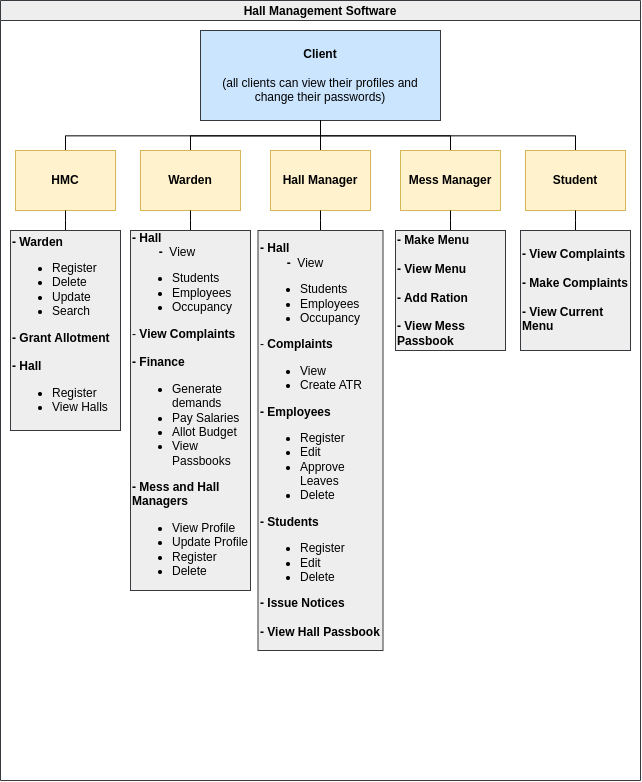
\includegraphics[width=1.0\linewidth]{Class_Functionalities.png}
    \caption{Classes and their functionalities}
    \label{fig:enter-label}
\end{figure}

\section{Hardware Interfaces}
\begin{enumerate}
    \item The hardware used for this needs to be server computer with a processor fast enough to handle a large number of requests simultaneously. Preferably a multi-core system with distributed processes across the core will be suitable.
    \item Solid state drives instead of hard disks to boost the speed of information retrieval. Enables faster request handling.
    \item RAID systems to manage data redundancy. Ensures no user data is lost because of storage device failures by maintaining redundant copies as backup.
\end{enumerate}
\section{Software Interfaces}
\begin{enumerate}
    \item A Web browser needed on the end-users' systems to access the web application
    \item Graphical user interfaces combined with the browsers needed. Command-line interface will not be able to meaningfully handle the user interfaces provided in the web application.
    \item In order to set up the system, some web server like Heroku may be needed for deployment.Currently the system runs on the local device of the user.
    \item The client will need an active email address for verification.
\end{enumerate}
\section{Communications Interfaces}
\begin{enumerate}
    \item The system uses a standard TCP/IP stack available on most operating systems.
    \item The system uses the \textbf{HTTP} protocol to deliver web pages and handle user login
\end{enumerate}

\chapter{System Features}

\section{User Registration/Deletion}
\subsection{HMC}
\subsubsection{Description}
    The HMC is created in the django admin page. This is to be created by the System maintainer.
\subsubsection{Stimulus/Response Sequences}
\begin{itemize}
    \item Stimulus: The college wishes to register a Hall management committee into the system
    \item Response: Maintainer can create an HMC from the django admin interface.
\end{itemize}
\subsubsection{Functional Requirements}
\begin{itemize}
    \item \textbf{REQ1}: Django admin authorisation
    \item \textbf{REQ2}: Digital form for creation of HMC with superuser privileges
\end{itemize}

\subsection{Hall}
\subsubsection{Description}
Halls along with there residence specifications can be created by the HMC. Only the HMC and the Warden has access to this page.
\subsubsection{Stimulus/Response Sequences}
\begin{itemize}
    \item Stimulus: A new Hall needs to be registered in the system.
    \item Response: System adds the hall and creates rooms in the database along with their specified rent and occupancy.
\end{itemize}
\begin{itemize}
    \item Stimulus: The status of the hall needs to be checked regarding occupancy.
    \item Response: System queries the database and displays the status of all rooms in the hall.
\end{itemize}

\subsubsection{Functional Requirements}
\begin{itemize}
    \item \textbf{REQ4}: Digital forms for the creation of halls.
    \item \textbf{REQ5}:  Automated filling of the database with room numbers based on the specifications provided regarding the blocks and floors.
    \item \textbf{REQ6}: Page to show the data of each hall based on the current and the maximum occupancy.
\end{itemize}
Clarity in occupancy of the hall makes it easier for the HMC to approximate allowable funds for the ration etc for the hall.

\subsection{Warden}
\subsubsection{Description}
Wardens can be allocated to halls by the HMC. The details can be added by a page only accessible to the HMC.
\subsubsection{Stimulus/Response Sequences}
\begin{itemize}
    \item Stimulus: HMC wishes to allocate a warden to the hall via the registration page.
    \item Response: The form needs to be filled and the email needs to be verified by the warden in order to activate their account.
\end{itemize}

\begin{itemize}
    \item Stimulus: HMC wishes to update the information for the allocated hall warden.
    \item Response: The database is queried and the data is pre-furnished in the form in order to update the data of the warden.
\end{itemize}

\begin{itemize}
    \item Stimulus: HMC wishes de-allocate a hall to a warden.
    \item Response: Confirmation page for the deletion for the warden. The system deletes the warden from the hall data.
\end{itemize}

\subsubsection{Functional Requirements}
\begin{itemize}
    \item \textbf{REQ7}: Digital forms for the registration and allocation of the wardens.
    \item \textbf{REQ8}: Email verification needs the existence of a unique email per each warden.
    \item \textbf{REQ9}: User authentication page before deletion of warden data.
\end{itemize}
Email verification provides 2-step authentication system for security. Security during the deletion of the registered hall warden ensures only authenticated users can de-allocate wardens from the hall.

\subsection{Hall/Mess manager}
\subsubsection{Description}
Wardens can appoint an register managers for their Hall. The details can be added by a page only accessible to the Warden.
\subsubsection{Stimulus/Response Sequences}
\begin{itemize}
    \item Stimulus: The warden wishes to allocate a manager to the hall via the registration page.
    \item Response: The form needs to be filled and the email needs to be verified by the manager in order to activate their account.
\end{itemize}

\begin{itemize}
    \item Stimulus: The warden wishes to update the information for the allocated manager.
    \item Response: The database is queried and the data is displayed pre-filled in the form in order to update the data of the manager.
\end{itemize}

\begin{itemize}
    \item Stimulus: Warden wishes to de-register a manager. 
    \item Response: Confirmation page for the deletion for the hall manager. The warden must enter their password before progressing for deletion.
\end{itemize}

\subsubsection{Functional Requirements}
\begin{itemize}
    \item \textbf{REQ10}: Digital forms for the registration and allocation of the manager.
    \item \textbf{REQ11}: Email verification needs the existence of a unique email per each manager.
    \item \textbf{REQ12}: User authentication page before deletion of manager data.
\end{itemize}
Email verification provides 2-step authentication system for security. Security during the deletion of the registered manager ensures only authenticated users can de-allocate managers from the hall.

\subsection{Students}
\subsubsection{Description}
Hall managers have access to the page to register the students in their halls. Like other registration pages, Email verification is mandated here as well for the students. Additionally, automated room allocation based on the preferences of the students is also possible.
\subsubsection{Stimulus/Response Sequences}
\begin{itemize}
    \item Stimulus: Hall management wishes to register students in the hall.
    \item Response: Students are added to the database on the form input via Email verification.
\end{itemize}

\begin{itemize}
    \item Stimulus: While registration, Student wishes to declare their room preferences.
    \item Response: Up to 3 room preference can be added in the form. The system will allocate one of the rooms of preference if available, otherwise a room is randomly allocated.
\end{itemize}

\begin{itemize}
    \item Stimulus: The manager wishes deletion of student data from the hall database.
    \item Response: Up to 3 room preference can be added in the form. The system will allocate one of the rooms of preference if available, otherwise a room is randomly allocated.
\end{itemize}

\subsubsection{Functional Requirements}
\begin{itemize}
    \item \textbf{REQ13}: Digital forms for the registration and room allocation for a student.
    \item \textbf{REQ14}: Email verification needs the existence of a unique email per each student.
    \item \textbf{REQ15}: Choices by a student can be filled in a priority ordering.
\end{itemize}
Deletion page enables the hall to clear the data of the student in the event of a hall re-allocation or graduation.

\subsection{Hall employees}
\subsubsection{Description}
Hall managers have access to the page to employ workers for the hall. As the hall employee is not a direct user of the  system, no email verification is needed here. Roles and salaries can be fixed during registering.
\subsubsection{Stimulus/Response Sequences}
\begin{itemize}
    \item Stimulus: Hall management wishes to employ a hall worker.
    \item Response: Page with personal details, job, salary bracket is furnished.
\end{itemize}

\subsubsection{Functional Requirements}
\begin{itemize}
    \item \textbf{REQ16}: Digital forms for the employee details to be furnished by the manager.
\end{itemize}
Salary brackets are currently restricted to a few limited options to be selected by the manager.

\section{Budget allocations}
\subsection{HMC}
\subsubsection{Description}
Grants may be allocated to the halls based at demand via a restricted page. The funds are added to the Warden's budget to manage from that point onwards. 
\subsubsection{Stimulus/Response Sequences}
\begin{itemize}
    \item Stimulus: Allocation of grants to the halls by the HMC.
    \item Response: The System renders the form for the allotment after validating user. Allotted budget is added to the warden passbook.
\end{itemize}
\subsubsection{Functional Requirements}
\begin{itemize}
    \item \textbf{REQ1}: Digital form for budget allocation.
    \item \textbf{REQ2}: Allocated budget is displayed in the passbook of the warden.
\end{itemize}

\subsection{Warden}
\subsubsection{Description}
The warden, upon receiving budget from  the HMC can decide how much allocation of funds is needed to the mess and the hall facilities respectively.
\subsubsection{Stimulus/Response Sequences}
\begin{itemize}
    \item Stimulus: Warden wants to distribute the funds to the mess and the hall.
    \item Response: System verifies the password of the user and proceeds to allocate the funds to the hall and the mess passbooks respectively.
\end{itemize}
\begin{itemize}
    \item Stimulus: Warden wishes to view the past allocations to the hall and mess.
    \item Response: The warden passbook page displays the past allotments with their timestamp
\end{itemize}

\subsubsection{Functional Requirements}
\begin{itemize}
    \item \textbf{REQ3}: Digital forms for the filing of action taken reports.
    \item \textbf{REQ4}: Passbook to display the past allocations both to and by the warden.
\end{itemize}

\section{Hall employee handling}
\subsection{Salaries}
\subsubsection{Description}
The warden is authorised to grant the salaries to the employees out of the hall budget. This is logged into the hall passbook.
\subsubsection{Stimulus/Response Sequences}
\begin{itemize}
    \item Stimulus: Salaries are to be paid to the hall employees. 
    \item Response: System verifies password of current logged in user. The page is available only to the hall warden.
\end{itemize}

\subsubsection{Functional Requirements}
\begin{itemize}
    \item \textbf{REQ1}: The salaries of each type of employee is queried and aggregated and added to the hall passbook along with the timestamp.
\end{itemize}
\subsection{Leaves}
\subsubsection{Description}
The hall manager can register the duration of permitted leave and whether or not the leave will be paid based upon documentary uploads.
\subsubsection{Stimulus/Response Sequences}
\begin{itemize}
    \item Stimulus: Hall employee leave requests need to be processed by the hall manager.
    \item Response: System loads the form for the hall manager and they can select the duration of the leave. Provision to upload any documents if needed also exists. 
\end{itemize}

\subsubsection{Functional Requirements}
\begin{itemize}
    \item \textbf{REQ2}: Ability to enter leaves of absence on a digital calendar.
    \item \textbf{REQ3}: Calculation of amount payable based on attendance.
    \item \textbf{REQ4}: If the leave is to be paid, The manager must upload a document in support of it.
\end{itemize}

\section{Fees and dues management}
\subsubsection{Description}
Students are to pay for the hall and the mess charges. Both the requests must be processed separately for easy tracking. These payments must be recorded and collected without irregularities.
\subsubsection{Stimulus/Response Sequences}
\begin{itemize}
    \item Stimulus: Students dues are to be generated and displayed to them.
    \item Response: The warden will generate dues to the student for both hall and mess charges separately. They must validate themselves first before generating this demand.
\end{itemize}

\begin{itemize}
    \item Stimulus: Student requests the total amount owed with different filters (such as mess, rent, common room fees, etc).
    \item Response: A web page with the relevant information is displayed.
\end{itemize}

\begin{itemize}
    \item Stimulus: Student wishes to clear the dues generated for him.
    \item Response: Payment portal is rendered where the student can pay their dues.
\end{itemize}
\subsubsection{Functional Requirements}
\begin{itemize}
    \item \textbf{REQ1}: Ability to track the dues owed by different students.
    \item \textbf{REQ2}: The request generation is password protected to avoid errors.
    \item \textbf{REQ3}: Stripe payment is used here. To customize the payment options, contact the developers.
    \item \textbf{REQ4}: Student passbook keeps a record of all the payments made by the student. This can be downloaded by the student in PDF format.
\end{itemize}


\section{Complaints management}
\subsection{Student}
\subsubsection{Description}
Students should be able to generate complaints and view the corresponding action taken reports (ATR).
\subsubsection{Stimulus/Response Sequences}
\begin{itemize}
    \item Stimulus: Student intents to register a complaint  
    \item Response: System loads the form for the student. The complaint details can be filled in a text format in the form. Provision to upload any images of the complaint if needed also exists. 
\end{itemize}

\subsubsection{Functional Requirements}
\begin{itemize}
    \item \textbf{REQ1}: The complaint details can be filled in a text format in the form.
    \item \textbf{REQ2}: Image format can be uploaded and viewed by the manager.
    \item \textbf{REQ3}: The ATR can be downloaded by the student if the issue has been resolved.
\end{itemize}

\subsection{Hall manager}
\subsubsection{Description}
The manager should be able to view the complaint and assign an employee to deal with it if needed. They should also be able generate an ATR if needed.
\subsubsection{Stimulus/Response Sequences}
\begin{itemize}
    \item Stimulus: Warden wishes to assign workers to deal with an issue raised by a student. 
    \item Response: The warden can enter the assigned worker and the details of the action taken in a text format. The status of the complaint then can be marked as completed or not accordingly by the manager. 
\end{itemize}

\subsubsection{Functional Requirements}
\begin{itemize}
    \item \textbf{REQ4}: The ATR details can be filled in a text format alomg with the status in the form.
    \item \textbf{REQ5}: PDF can be generated by the manager, which cam be downloaded by the student.
\end{itemize}

\section{Hall notices}
\subsection{Hall Manager}
\subsubsection{Description}
The hall manager must have the option of adding notices in order to notify each student of the hall.
\subsubsection{Stimulus/Response Sequences}
\begin{itemize}
    \item Stimulus: Hall manager intends to add notices.
    \item Response: A form that allows the hall manager to upload images and text based notices which will show up on the pages of each of the student which reside in that hall.
\end{itemize}

\subsubsection{Functional Requirements}
\begin{itemize}
    \item \textbf{REQ1}: Ability to add text to the notice.
    \item \textbf{REQ2}: Ability to upload images to the notice board.
    \item \textbf{REQ3}: The hall manager and the warden should be able to preview the uploaded notice.
\end{itemize}

\subsection{Student}
\subsubsection{Description}
All the students should be able to view the notices uploaded by the hall management.
\subsubsection{Stimulus/Response Sequences}
\begin{itemize}
    \item Stimulus: Students intends to view the hall notice board.
    \item Response: The student can navigate to the notice board page post login.
\end{itemize}

\subsubsection{Functional Requirements}
\begin{itemize}
    \item \textbf{REQ4}: Access the notice board with only view only permissions.
\end{itemize}

\section{Mess Management}
\subsection{Menu}
\subsubsection{Description}
Mess managers can perform various functions like generating the monthly mess menu.
\subsubsection{Stimulus/Response Sequences}
\begin{itemize}
    \item Stimulus: Mess manager wishes to generate the mess menu for the month.
    \item Response: The system generates a form for a week as menus are weekly based in halls. Here the mess manger can set the fields for 4 meals a day, 7 days a week.
\end{itemize}
\begin{itemize}
    \item Stimulus: The student wishes to view the mess menu generated.
    \item Response: The system fetches the menu database and filters and displays the menu based on thew hall of the student.
\end{itemize}

\subsubsection{Functional Requirements}
\begin{itemize}
    \item \textbf{REQ1}: Both the student and mess manager can view the mess menu in a neat tabulated manner.
    \item \textbf{REQ2}: Only the mess manager is granted access to the menu editing page.
\end{itemize}

\subsection{Rations and Mess passbook}
\subsubsection{Description}
The mess manager can log the rations used on a daily basis
\subsubsection{Stimulus/Response Sequences}
\begin{itemize}
    \item Stimulus: Mess manager intends to add the ration used per day.
    \item Response: The system generates the form to .
\end{itemize}
\begin{itemize}
    \item Stimulus: Mess manager wishes to view the expenditure of the mess.
    \item Response: The mess passbook page enables the mess manager to view and download the rations consumed in PDF format.
\end{itemize}
\subsubsection{Functional Requirements}
\begin{itemize}
    \item \textbf{REQ3}: The aggregate price of the rations are calculated and added to the mess passbook automatically.
    \item \textbf{REQ4}: The mess passbook is neatly tabulated and the expenses are labelled according to their nature.
\end{itemize}

\section{Hall Expense Report}
\subsection{Description}
Wardens need to view the cash flow and various expenses owed. This information needs to be quickly retrieved without having to go through paper records. Mess fees, rent, grants, etc, can be centralized in a single location for the warden to review.
\subsection{Stimulus/Response Sequences}
\begin{itemize}
    \item Stimulus: Warden requests various expenses.
    \item Response: A form that allows the warden to apply various filters is displayed. Based on the form input, the expenses database is filtered and the relevant information is presented, such as the amount of owed by students, amount owed to mess managers, etc.
\end{itemize}

\begin{itemize}
    \item Stimulus: Warden requests a full accounting report
    \item Response: The system produces a table with all the expenses and payments accounted for. Cheques will automatically be generated. Warden will be able to print this report and the generated cheques.
\end{itemize}
\subsubsection{Functional Requirements}
\begin{itemize}
    \item \textbf{REQ17}: Ability to generate accounting reports
    \item \textbf{REQ18}: Ability to generate cheques.
    \item \textbf{REQ19}: Ability to submit the generated reports for audit.
\end{itemize}

\chapter{Other Nonfunctional Requirements}

\section{Performance Requirements}
\subsection{Server Up-time}
The system needs to keep running for long periods of time for accessibility so the hardware needs to be capable of that. Moreover the maintenance frequency needs to be low to have a stable experience for the end users.\subsection{Response Time}
The system needs to have a good response time as it will be repetitively used by various stakeholders in the Institute and the response time needs to keep up with the incoming requests. At the same time less used tasks like printing bills at the end of the month can be a little slow since they will be accessed much less frequently.
\subsection{System Dependability}
It determines the failure rate of the system, that is, the cases when the system receives an incorrect input or there is a random failure. The end user needs to be notified in such a scenario.
\subsection{Prominent Documents}
Since the system is also being used to maintain cash receipts and expenditure through the halls and generate official documents for the students' stay in their halls, the output needs to be clear, concise and consistent in a .pdf or another similar printable format.



\section{Safety Requirements}
There needs to be a regular audit to the cash flow through the hall since there is no check for the information entered by the mess manager. Moreover, audit also needs to be done for the budget distribution as there might be cases for fraud in the long run if left unchecked since the system is not verifying the data in any manner.

\section{Security Requirements}
\subsection{Secure Login}
The system should be protected against forced and malicious login attempts to access the software. The web interface needs to be continuously patched to fix bugs as and when they crop up.
\subsection{Verifiable Access}
The system is designed to serve multiple parties and their levels of access and their permissions are decided by their login IDs. Thus, the login and access to functionality should be robust and extremely secure since the system also deals with the finances of the institute.
\subsection{Student Information Must be Secure}
All the personal student information stored by the system should be safe and secure.

\section{Software Quality Attributes}
\subsection{Reliability}
The system must be dependable, which means it must constantly perform as expected with very low downtime and rate of failure. In absence of this the HCM will not be able to function smoothly.
\subsection{Information Accessibility}
To save the login credentials and the myriad types of data that the software uses, the application should be able to save, access and alter files on the system so that the information is retained even on successive runs.
\subsection{Maintainability}
The program should be easy to modify and add features to. The code should be clearly commented and the features well documented to allow for easy maintenance. The frameworks used should be well supported by their developers well into the future.

\end{document}